\chapter{System Architecture and Implementation}
\label{ch:system-architecture}

The AquaTrack implementation is organized as a layered mobile health system. The architecture begins with multimodal sensing, continues through preprocessing and dual-pipeline prediction, and ends with backend inference and mobile visualization. This modular structure allows the sensing prototype, data-processing workflow, and deployment interface to be improved independently.

\section{System Architecture}

The AquaTrack framework is conceptualized as a context-aware, multimodal mobile health (m-health) system designed to deliver robust dehydration risk assessments. The architecture follows a modular, layered paradigm that facilitates end-to-end data integrity -- from high-fidelity physiological acquisition to real-time mobile visualization. By integrating biochemical sensing with environmental context, the system achieves a level of adaptive inference necessary for practical wearable deployment.

Figure \ref{fig:aquatrack-architecture} provides a high-level overview of the integrated AquaTrack ecosystem. The architecture is designed to handle the complexities of multimodal physiological data while ensuring low-latency inference and high user engagement through its layered organizational approach.

\section{Preprocessing and Feature Engineering Pipeline}

The Data Engineering Pipeline enforces preprocessing consistency and prevents downstream data leakage. It implements a sequential workflow involving column-wise median imputation for missing data recovery, winsorization for outlier suppression, and logarithmic transformation to stabilize high-variance biomarker distributions. Feature normalization is achieved through robust scaling, utilizing the interquartile range to maintain sensitivity to physiological shifts while remaining resilient to sensor noise. The engineered outputs include interaction-aware composite biomarkers which map raw data to clinically relevant indices of fluid depletion.

\section{Context Detection and ML Inference Layer}

Th Context Detection layer is the one which performs real-time activity analysis and climate classification. This module estimates the reliability of the biomarker readings by evaluating the sweat availability and the user's metabolic state, effectively acting as an adaptive gain-control for the prediction engine. In low-sweat or sedentary states, the system shifts its inferential weight towards context-driven indicators, whereas in high-exertion states, it prioritizes the biochemical evidence.

The ML Inference Layer utilizes a dual-pipeline architecture to process biomarker and context features independently. Each pipeline employs high-performance models, which are optimized through stratified k-fold cross-validation, hyperparameter tuning and macro F1 maximization. The final dehydration risk score is derived through a weighted fusion strategy, ensuring that the categorical risk labels (Low, Medium, High) are grounded in both physiological truth and environmental reality.

\section{Backend and Mobile Deployment}

To ensure deployment feasibility, the prediction framework is served via a RESTful API architecture built on the FastAPI framework. The backend manages the lifecycle of serialized model artifacts (.pkl), receiving structured JSON payloads from the wearable unit and returning low-latency risk predictions. This backend-driven approach allows for centralized model updates and complex inference without taxing the wearable hardware's limited computational resources.

The user interface is implemented as a React Native iOS dashboard, providing a real-time visualization of the user's hydration trajectory. The mobile application translates complex model outputs into actionable health insights, including trend monitoring, personalized alerts, and hydration recommendations. By connecting laboratory-grade sensing with a modern mobile interface, the AquaTrack architecture demonstrates a scalable pathway for next-generation hydration monitoring in diverse real-world settings.

\begin{figure}[htb]
\centering
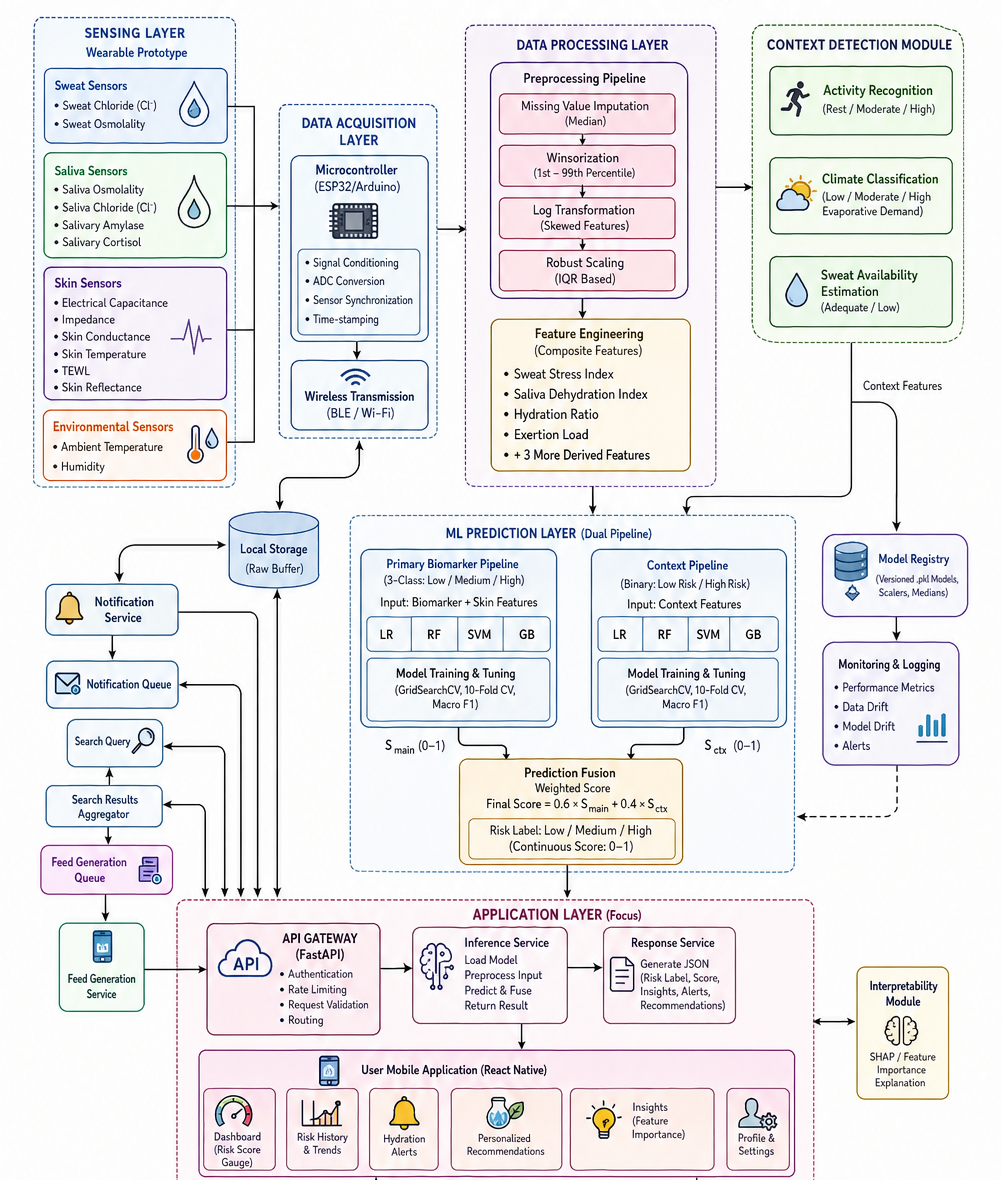
\includegraphics[width=0.85\textwidth]{Figures/aquatrack/image7}
\caption{End-to-end modular system architecture for AquaTrack}
\label{fig:aquatrack-architecture}
\end{figure}